%%%%%%%%%%%%%%%%%%%%%%%%%%%%%%%%%%%%%%%%%%%%%%%%%%%%%%%%%%%%%%%%%%%%%%%%%%%%%%%%
%%%%%%%%%%%%%%%%%%%%%%%%%%%%%%%%%%%%%%%%%%%%%%%%%%%%%%%%%%%%%%%%%%%%%%%%%%%%%%%%
\exercice{Décomposition en signaux usuels}
%%%%%%%%%%%%%%%%%%%%%%%%%%%%%%%%%%%%%%%%%%%%%%%%%%%%%%%%%%%%%%%%%%%%%%%%%%%%%%%%
%%%%%%%%%%%%%%%%%%%%%%%%%%%%%%%%%%%%%%%%%%%%%%%%%%%%%%%%%%%%%%%%%%%%%%%%%%%%%%%%

%%%%%%%%%%%%%%%%%%%%%%%%%%%%%%%%%%%%%%%%%%%%%%%%%%%%%%%%%%%%%%%%%%%%%%%%%%%%%%%%
\question{}
%%%%%%%%%%%%%%%%%%%%%%%%%%%%%%%%%%%%%%%%%%%%%%%%%%%%%%%%%%%%%%%%%%%%%%%%%%%%%%%%
\tikzsetnextfilename{ex1_1_corrige-chap0-ext}
\begin{center}
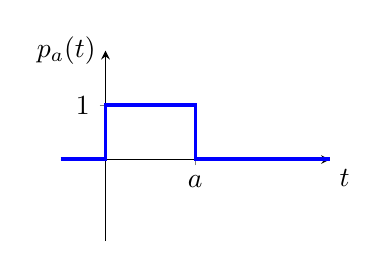
\begin{tikzpicture}
   \begin{axis}[
   height=4cm,
   width=5cm,
      axis x line=center,
        axis y line=center,
        xmin=-1,
        xmax=5,
        ymin=-1.5,
        ymax=2.0,
        xlabel={$t$},
        ylabel={$p_a(t)$},
        xlabel style={below right},
        ylabel style={left},
        yticklabels={1},
        ytick={1},
        y tick label style={anchor=east},
        xticklabels={$a$},
        xtick={2},
        x tick label style={anchor=north},
        ]
        \addplot [very thick,color=blue,const plot]  
        coordinates { (-1,0.01) (0,0.01) (0,1) (2,1)  (2,0.01) (5,0.01) };
        \end{axis}
\end{tikzpicture}
\tikzsetnextfilename{ex1_2_corrige-chap0-ext}
\begin{tikzpicture}
   \begin{axis}[
   height=4cm,
   width=5cm,
      axis x line=center,
        axis y line=center,
        xmin=-1,
        xmax=5,
        ymin=-1.5,
        ymax=2.0,
        xlabel={$t$},
        ylabel={$p_a(t)$},
        xlabel style={below right},
        ylabel style={left},
        yticklabels={1},
        ytick={1},
        y tick label style={anchor=east},
        xticklabels={$a$},
        xtick={2},
        x tick label style={below left},
        ]
        \addplot [very thick,color=col4,const plot]   
        coordinates { (-1, 0.01) (0, 0.01) (0 ,1)  (5,1) };
        \addplot [very thick,color=col3,const plot] 
        coordinates { (-1,-0.01) (0,-0.01) (2,-1) (5,-1) };
        \end{axis}
\end{tikzpicture}
\end{center}
$$
\color{blue}p_a(t)=\color{col4}u(t)\color{col3}-u(t-a)
$$ 
où $u(t)$ est la fonction échelon unité.

On rappel la transformée de Laplace d'une fonction retardée :
$$
\laplace{f(t-\tau)} = e^{-\tau p}F(p)
$$
La transformée de Laplace de $p_a(t)$ est donnée par : 
$$
P_a(p) = \laplace{p_a(t)}=\laplace{u(t)}-\laplace{u(t-a)}
=\dfrac{1}{p}(1-e^{-a p})
$$

%%%%%%%%%%%%%%%%%%%%%%%%%%%%%%%%%%%%%%%%%%%%%%%%%%%%%%%%%%%%%%%%%%%%%%%%%%%%%%%%
\question{}
%%%%%%%%%%%%%%%%%%%%%%%%%%%%%%%%%%%%%%%%%%%%%%%%%%%%%%%%%%%%%%%%%%%%%%%%%%%%%%%%

\tikzsetnextfilename{ex1_3_corrige-chap0-ext}
\begin{center}
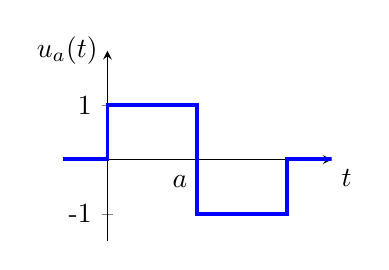
\begin{tikzpicture}
   \begin{axis}[
   height=4cm,
   width=5cm,
      axis x line=center,
        axis y line=center,
        xmin=-1,
        xmax=5,
        ymin=-1.5,
        ymax=2.0,
        xlabel={$t$},
        ylabel={$u_a(t)$},
        xlabel style={below right},
        ylabel style={left},
        yticklabels={-1,1},
        ytick={-1,1},
        y tick label style={anchor=east},
        xticklabels={$a$},
        xtick={2},
        x tick label style={below left},
        ]
        \addplot [very thick,color=blue,const plot] coordinates 
        {(-1,0.01) (0,0.01) (0,1) (2,1)  (2,-1) (4,-1) (4,0.01) (5,0.01)};
        \end{axis}
\end{tikzpicture}
\tikzsetnextfilename{ex1_4_corrige-chap0-ext}
\begin{tikzpicture}
   \begin{axis}[
    height=4cm,
    width=5cm,
    axis x line=center,
    axis y line=center,
    xmin=-1,
    xmax=5,
    ymin=-1.5,
    ymax=2.0,
    xlabel={$t$},
    ylabel={$u_a(t)$},
    xlabel style={below right},
    ylabel style={left},
    yticklabels={-1,1},
    ytick={-1,1},
    y tick label style={anchor=east},
    xticklabels={$a$},
    xtick={2},
    x tick label style={below left},
    ]
    \addplot[very thick,color=col4,const plot]    
    coordinates { (-1, 0.01) (0, 0.01) (0,1)  (2 ,1) (2, 0.01) (5,0.01) };
    \addplot[very thick,color=col3,const plot]  
    coordinates { (-1,-0.01) (2,-0.01) (2,-1) (4,-1) (4,-0.01) };
    \end{axis}
\end{tikzpicture}
\end{center}
$$
\color{blue}u_a(t)=\color{col4}p_a(t)\color{col3}-p_a(t-a)
$$ 
où $p_a(t)$ est la fonction fonction porte construite précédemment.

La transformée de Laplace de $u_a(t)$ est donnée par :
$$
U_a(p)=\laplace{u_a(t)}=\laplace{p_a(t)}-\laplace{p_a(t-a)}
      =P_a(p)(1-e^{-a p})=\dfrac{(1-e^{-ap})^2}{p}
$$

%%%%%%%%%%%%%%%%%%%%%%%%%%%%%%%%%%%%%%%%%%%%%%%%%%%%%%%%%%%%%%%%%%%%%%%%%%%%%%%%
\question{}
%%%%%%%%%%%%%%%%%%%%%%%%%%%%%%%%%%%%%%%%%%%%%%%%%%%%%%%%%%%%%%%%%%%%%%%%%%%%%%%%

\tikzsetnextfilename{ex1_5_corrige-chap0-ext}
\begin{center}
\begin{tikzpicture}
    \begin{axis}[
    height=4cm,
    width=5cm,
    axis x line=center,
    axis y line=center,
    xmin=-1,
    xmax=5,
    ymin=-1.5,
    ymax=2.0,
    xlabel={$t$},
    ylabel={$g_0(t)$},
    xlabel style={below right},
    ylabel style={above left},
    yticklabels={$E$},
    ytick={1},
    y tick label style={left},
    xticklabels={$\dfrac{T}{2}$,$T$},
    xtick={2,4},
    x tick label style={below},
    ]
    \addplot[very thick,color=blue,domain=-1:0, samples=101]{0.05};
    \addplot[very thick,color=blue,domain=0:2, samples=101]{0.5*x};
    \addplot [very thick,color=blue,domain=2:4, samples=101]{-0.5*x+2};
    \addplot [very thick,color=blue,domain=4:5, samples=101]{0.05};
    \end{axis}
\end{tikzpicture}
\tikzsetnextfilename{ex1_6_corrige-chap0-ext}
\begin{tikzpicture}
    \begin{axis}[
    height=4cm,
    width=5cm,
    axis x line=center,
    axis y line=center,
    xmin=-1,
    xmax=5,
    ymin=-1.5,
    ymax=2.0,
    xlabel={$t$},
    ylabel={$\frac{\mathrm{d}g_0(t)}{\mathrm{d}t}$},
    xlabel style={below right},
    ylabel style={above left},
    yticklabels={$\dfrac{2E}{T}$},
    ytick={1},
    y tick label style={left},
    xticklabels={$\dfrac{T}{2}$,$T$},
    xtick={2,4},
    x tick label style={below},
    ]
    \addplot [very thick,color=blue,domain=-1:0, samples=101]{0.01};
    \addplot [very thick,color=blue,domain=0:2, samples=101]{1.0};
    \addplot [very thick,color=blue,domain=2:4, samples=101]{-1.0};
    \addplot [very thick,color=blue,domain=4:5, samples=101]{0.01};
    \end{axis}
\end{tikzpicture}
\end{center}
$$
g_0(t)=\dfrac{2E}{T}\int_{0}^{t}u_{T/2}(t)\,\,\mathrm{d}\tau
$$

On rappel la transformée de Laplace de l'intégrale d'une fonction:
$$
\laplace{\int_{0}^{t}f(t)\,\,\mathrm{d}\tau}=\dfrac{F(p)}{p}
$$


La transformée de Laplace de $g_0(t)$ est donnée par :
$$
G_0(p) = \laplace{g_0(t)}=\dfrac{2E}{T}\dfrac{(1-e^{-Tp/2})^2}{p^2}
$$

%%%%%%%%%%%%%%%%%%%%%%%%%%%%%%%%%%%%%%%%%%%%%%%%%%%%%%%%%%%%%%%%%%%%%%%%%%%%%%%%
%%%%%%%%%%%%%%%%%%%%%%%%%%%%%%%%%%%%%%%%%%%%%%%%%%%%%%%%%%%%%%%%%%%%%%%%%%%%%%%%
\exercice{Décomposition en signaux usuels (2)}
%%%%%%%%%%%%%%%%%%%%%%%%%%%%%%%%%%%%%%%%%%%%%%%%%%%%%%%%%%%%%%%%%%%%%%%%%%%%%%%%
%%%%%%%%%%%%%%%%%%%%%%%%%%%%%%%%%%%%%%%%%%%%%%%%%%%%%%%%%%%%%%%%%%%%%%%%%%%%%%%%

%%%%%%%%%%%%%%%%%%%%%%%%%%%%%%%%%%%%%%%%%%%%%%%%%%%%%%%%%%%%%%%%%%%%%%%%%%%%%%%%
%%%%%%%%%%%%%%%%%%%%%%%%%%%%%%%%%%%%%%%%%%%%%%%%%%%%%%%%%%%%%%%%%%%%%%%%%%%%%%%%
\exercice{\'Etude d'équations différentielles}
%%%%%%%%%%%%%%%%%%%%%%%%%%%%%%%%%%%%%%%%%%%%%%%%%%%%%%%%%%%%%%%%%%%%%%%%%%%%%%%%
%%%%%%%%%%%%%%%%%%%%%%%%%%%%%%%%%%%%%%%%%%%%%%%%%%%%%%%%%%%%%%%%%%%%%%%%%%%%%%%%

%%%%%%%%%%%%%%%%%%%%%%%%%%%%%%%%%%%%%%%%%%%%%%%%%%%%%%%%%%%%%%%%%%%%%%%%%%%%%%%%
\question{}
%%%%%%%%%%%%%%%%%%%%%%%%%%%%%%%%%%%%%%%%%%%%%%%%%%%%%%%%%%%%%%%%%%%%%%%%%%%%%%%%
La première équation différentielle dans le domaine de Laplace, donne : 
\begin{align*}
p^2S(p)+110pS(p)+1000S(p)=pX(p)+30X(p) \\
S(p) ( p^2+110p+1000) = (p+30)X(p) \\
S(p) = \dfrac{(p+30)}{(p^2+110p+1000)} X(p) 
\end{align*}
cette dernière expression est de la forme :
\begin{align}
S(p) = H_2(p) X(p)
\label{eq-h2}
\end{align}
où $H_2(p)$ est une fonction de transfert d'un SLCI d'entrée $X(p)$ 
et de sortie $S(p)$.
\begin{center}
\tikzsetnextfilename{ex_2_corrige-chap0-ext}
\begin{tikzpicture}
    \sbEntree{E}
    \sbBloc[3]{H2}{$H_2(p)=\dfrac{(p+30)}{(p^2+110p+1000)}$}{E}
        \sbRelier[$X(p)$]{E}{H2}
    \sbSortie[3]{S}{H2}
        \sbRelier[$S(p)$]{H2}{S}
\end{tikzpicture}
\end{center}

La seconde équation différentielle, dans le domaine de Laplace, donne : 
\begin{align*}
    pX(p)+X(p)=KE(p) \\
    X(p) (p+1) = KE(p) \\
    X(p) = \dfrac{K}{(p+1)} E(p) 
\end{align*}
cette dernière expression est de la forme :
\begin{align}
X(p) = H_1(p) E(p)
\label{eq-h1}
\end{align}
où $H_2(p)$ est une fonction de transfert d'un SLCI d'entrée $E(p)$ 
et de sortie $X(p)$ :
\begin{center}
\tikzsetnextfilename{ex2_2_corrige-chap0-ext}
\begin{tikzpicture}
    \sbEntree{E}
    \sbBloc[3]{H1}{$H_1(p)=\dfrac{K}{(p+1)}$}{E}
        \sbRelier[$E(p)$]{E}{H1}
    \sbSortie[3]{S}{H1}
        \sbRelier[$X(p)$]{H1}{S}
\end{tikzpicture}
\end{center}

%%%%%%%%%%%%%%%%%%%%%%%%%%%%%%%%%%%%%%%%%%%%%%%%%%%%%%%%%%%%%%%%%%%%%%%%%%%%%%%%
\question{}
%%%%%%%%%%%%%%%%%%%%%%%%%%%%%%%%%%%%%%%%%%%%%%%%%%%%%%%%%%%%%%%%%%%%%%%%%%%%%%%%
Tracer le schéma fonctionnel complet du système
\begin{center}
\tikzsetnextfilename{ex_2_3_corrige-chap0-ext}
\begin{tikzpicture}
    \sbEntree{E}
    \sbBloc[3]{H1}{$H_1(p)$}{E}
    \sbRelier[$E(p)$]{E}{H1}
    \sbBloc[3]{H2}{$H_2(p)$}{H1}
    \sbRelier[$X(p)$]{H1}{H2}
    \sbSortie[3]{S}{H2}
    \sbRelier[$S(p)$]{H2}{S}
\end{tikzpicture}
\end{center}

%%%%%%%%%%%%%%%%%%%%%%%%%%%%%%%%%%%%%%%%%%%%%%%%%%%%%%%%%%%%%%%%%%%%%%%%%%%%%%%%
\question{}
%%%%%%%%%%%%%%%%%%%%%%%%%%%%%%%%%%%%%%%%%%%%%%%%%%%%%%%%%%%%%%%%%%%%%%%%%%%%%%%%
%Déterminer la fonction de transfert du système.
A partir des equations \ref{eq-h2} et \ref{eq-h1}, on peut écrire :
$$
S(p) = H_2(p) H_1(p) E(p)
$$
On a alors une expression de la forme $S(p) =H(p) E(p)$,
avec $H(p)=H_2(p) H_1(p)=\dfrac{K(p+30)}{(p^2+110p+1000)(p+1)}$
\begin{center}
\tikzsetnextfilename{ex_2_4_corrige-chap0-ext}
\begin{tikzpicture}
\sbEntree{E}
\sbBloc[3]{H1}{$H(p)=H_2(p) H_1(p)$}{E}
\sbRelier[$E(p)$]{E}{H1}
\sbSortie[3]{S}{H1}
\sbRelier[$S(p)$]{H1}{S}
\end{tikzpicture}
\end{center}
On sollicite le système avec un échelon $e(t)=E_0 u(t)$

%%%%%%%%%%%%%%%%%%%%%%%%%%%%%%%%%%%%%%%%%%%%%%%%%%%%%%%%%%%%%%%%%%%%%%%%%%%%%%%%
\question{}
%%%%%%%%%%%%%%%%%%%%%%%%%%%%%%%%%%%%%%%%%%%%%%%%%%%%%%%%%%%%%%%%%%%%%%%%%%%%%%%%
%Déterminer la valeur finale de la sortie et la tangente à l'origine.
La valeur finale peut être obtenue par la propriété de la transformée 
de Laplace que l'on nomme le théorème de la valeur finale:
$$
\lim\limits_{t \rightarrow +\infty} f(t) = \lim\limits_{p \rightarrow 0} pF(p)
$$
dans le cas où le système précédent est sollicité par un échelon:
$$
pS(p)=\dfrac{KE_0(p+30)}{(p^2+110p+1000)(p+1)}
$$
$$
\lim\limits_{t \rightarrow +\infty} s(t) = \lim\limits_{p \rightarrow 0} pS(p) 
                                         = \dfrac{3}{100}KE_0
$$
pour déterminer la tangente à l'origine on applique le théorème de la valeur 
initiale à la dérivée du signal.
$$
\lim\limits_{t \rightarrow 0} \devi{s(0)}{} = 
\lim\limits_{p \rightarrow +\infty} p^2S(p))= 0
$$
la tangente de $s(t)$ est donc horizontal en 0.


%%%%%%%%%%%%%%%%%%%%%%%%%%%%%%%%%%%%%%%%%%%%%%%%%%%%%%%%%%%%%%%%%%%%%%%%%%%%%%%%
\question{}
%%%%%%%%%%%%%%%%%%%%%%%%%%%%%%%%%%%%%%%%%%%%%%%%%%%%%%%%%%%%%%%%%%%%%%%%%%%%%%%%
%Déterminer la sortie $s(t)$ et tracer le signal.
Pour déterminer le signal de sortie $s(t)$, nous allons appliquer la 
transformée de Laplace inverse sur :
$$
S(p) = \dfrac{KE_0(p+30)}{(p^2+110p+1000)(p+1)p}
$$
pour celà nous allons décomposer en élément simple cette fraction rationnelle. 
Le polynôme $p^2+110p+1000$ admet comme racine $p_1=-10$ et $p_2=-100$. 
On peut donc récrire : 
$$
S(p)=\dfrac{KE_0(p+30)}{p(p+1)(p+10)(p+100)}
$$
décomposons $S(p)$ de la manière suivante:
$$
S(p)=\dfrac{A}{p}+\dfrac{B}{p+1}+\dfrac{C}{p+10}+\dfrac{D}{p+100}
$$

les différents coefficients $A$,$B$,$C$ et $D$ peuvent être déterminés par 
les limites suivantes :

\begin{align*}
    A&=\lim\limits_{p \rightarrow 0} p S(p) = 
    \lim\limits_{p \rightarrow 0} 
    \dfrac{KE_0(p+30)}{(p+1)(p+10)(p+100)} =
    \dfrac{3}{100}KE_0 \\
    B&=\lim\limits_{p \rightarrow -1} (p+1) S(p) = 
    \lim\limits_{p \rightarrow -1} 
    \dfrac{KE_0(p+30)}{p(p+10)(p+100)}=
    -\dfrac{29}{891}KE_0\\
    C&=\lim\limits_{p \rightarrow -10} (p+10) S(p) = 
    \lim\limits_{p \rightarrow -10} 
    \dfrac{KE_0(p+30)}{p(p+1)(p+100)}=
    \dfrac{1}{405}KE_0 \\
    D&=\lim\limits_{p \rightarrow -100} (p+100) S(p) = 
    \lim\limits_{p \rightarrow -100} 
    \dfrac{KE_0(p+30)}{p(p+1)(p+10)}=
    \dfrac{7}{89100}KE_0 
\end{align*}

$$
S(p) = KE_0\left(\dfrac{3}{100}  \dfrac{1}{p} -\dfrac{29}{891}\dfrac{1}{p+1} +
                                 \dfrac{1}{405}\dfrac{1}{p+10} + 
                                 \dfrac{7}{89100}\dfrac{1}{p+100} \right)
$$

$$
s(t) = \laplacei{S(p)} = KE_0u(t)\left(\dfrac{3}{100} - 
                         \dfrac{29}{891}e^{-t}+\dfrac{1}{405}e^{-10t}+
                         \dfrac{7}{89100}e^{-100t} \right) 
$$
on vérifie que $s(+\infty)=\dfrac{3}{100}KE_0$, $s(0)=0$ et $\devi{s(0)}{}=0$
\begin{center}
\tikzsetnextfilename{ex_2_5_corrige-chap0-ext}
    \begin{tikzpicture}
        \begin{axis}[
        scaled y ticks = false,
        height=5cm,
        width=9cm,  
        axis x line=center,
        axis y line=center,
        xmin=-0.5,
        xmax=5,
        ymin=-0.01,
        ymax=0.04,
        xlabel={$t$},
        ylabel={$s(t)$},
        xlabel style={below right},
        ylabel style={left},
        yticklabels={0,$\dfrac{3}{100}KE_0$},
        ytick={0,0.03},
        y tick label style={anchor=east}
        ]

        \addplot [very thick,color=blue,domain=0:10, samples=501]  
        {3/100-29/891*exp(-x)+1/405*exp(-10*x)+7/89100*exp(-100*x)};
        \end{axis}
    \end{tikzpicture}
\end{center}


\newpage
%%%%%%%%%%%%%%%%%%%%%%%%%%%%%%%%%%%%%%%%%%%%%%%%%%%%%%%%%%%%%%%%%%%%%%%%%%%%%%%%
%%%%%%%%%%%%%%%%%%%%%%%%%%%%%%%%%%%%%%%%%%%%%%%%%%%%%%%%%%%%%%%%%%%%%%%%%%%%%%%%
\exercice{Fonction de transfert, réponse temporelle}
%%%%%%%%%%%%%%%%%%%%%%%%%%%%%%%%%%%%%%%%%%%%%%%%%%%%%%%%%%%%%%%%%%%%%%%%%%%%%%%%
%%%%%%%%%%%%%%%%%%%%%%%%%%%%%%%%%%%%%%%%%%%%%%%%%%%%%%%%%%%%%%%%%%%%%%%%%%%%%%%%

%%%%%%%%%%%%%%%%%%%%%%%%%%%%%%%%%%%%%%%%%%%%%%%%%%%%%%%%%%%%%%%%%%%%%%%%%%%%%%%%
%%%%%%%%%%%%%%%%%%%%%%%%%%%%%%%%%%%%%%%%%%%%%%%%%%%%%%%%%%%%%%%%%%%%%%%%%%%%%%%%
\question{}
%%%%%%%%%%%%%%%%%%%%%%%%%%%%%%%%%%%%%%%%%%%%%%%%%%%%%%%%%%%%%%%%%%%%%%%%%%%%%%%%
%%%%%%%%%%%%%%%%%%%%%%%%%%%%%%%%%%%%%%%%%%%%%%%%%%%%%%%%%%%%%%%%%%%%%%%%%%%%%%%%
\textbf{\tbf{(1) $\devi{s(t)}{}+2s(t)=e(t)$ avec $s(0)=2$ et $e(t)=e^{-t}$}}

La transformée de Laplace de l'équation différentielle donne :
\begin{align*}
    pS(p)-2+2S(p)&=E(p)\\
    S(p)&=\dfrac{1}{p+2}E(p)+\dfrac{2}{p+2}
\end{align*}
La fonction de transfert est le rapport de la sortie et de l'entrée lorsque 
les CI sont nulles, ici :
$$
H(p)=\dfrac{1}{p+2}
$$
pour $e(t)=e^{-t}$, $E(p)=\dfrac{1}{(p+1)}$ on peut alors écrire :
$$
S(p)=\dfrac{1}{(p+1)(p+2)}+\dfrac{2}{p+2}
$$
la transformée inverse donne :
$$
s(t) = \laplacei{S(p)}=e^{-t}-e^{-2t}+2e^{-2t}=e^{-t}+e^{-2t}
$$
\begin{center}
    \tikzsetnextfilename{ex_3_1_corrige-chap0-ext}
    \begin{tikzpicture}
    \begin{axis}
    [   scaled y ticks = false,
        height=5cm,
        width=10cm,
        axis x line=center,
        axis y line=center,
        xmin=-0.5,
        xmax=3.1,
        ymin=-0.01,
        ymax=3.0,
        xlabel={$t$},
        ylabel={$s(t)$},
        xlabel style={below right},
        ylabel style={left},
        yticklabels={0,$s(0)=2$},
        ytick={0,2.0},
        xtick={0,1,2,3},
        xticklabels={0,1,2,3},
        y tick label style={anchor=east}
    ]
    \addplot [signalb,domain=0:10 ] {exp(-x)+exp(-2*x)};
    \addplot [envelop,domain=0:10] {exp(-x)};
    \end{axis}
    \end{tikzpicture}
\end{center}

\newpage
%%%%%%%%%%%%%%%%%%%%%%%%%%%%%%%%%%%%%%%%%%%%%%%%%%%%%%%%%%%%%%%%%%%%%%%%%%%%%%%%
\question{}
%%%%%%%%%%%%%%%%%%%%%%%%%%%%%%%%%%%%%%%%%%%%%%%%%%%%%%%%%%%%%%%%%%%%%%%%%%%%%%%%
\tbf{(2)$\devi{s(t)}{2}+3\devi{s(t)}{}+2s(t)=\devi{e(t)}{} + e(t)$ 
avec $\devi{s(0)}{}=s(0)=0$ et $e(t) = e^{-3t}$}}
La transformée de Laplace de l'équation différentielle donne :
\begin{align*}
    p^2S(p)+3pS(p)+2S(p)&=pE(p)+E(p)\\
    S(p)(p^2+3p+2)&=(p+1)E(p)\\
    S(p) &= \dfrac{p+1}{p^2+3p+2}E(p)
\end{align*}
La fonction de transfert est donné par la fraction rationnelle :
$$
H(p)=\dfrac{p+1}{p^2+3p+2}
$$
les pôles de $H(p)$ sont $p_1=-2$ et $p_2=-1$, on peut donc factoriser la 
relation précédente par les pôles :
$$
S(p) = \dfrac{p+1}{(p+1)(p+2)}E(p)=\dfrac{1}{(p+2)}E(p)
$$
pour $e(t)=e^{-3t}$, $E(p)=\dfrac{1}{p+3}$
$$
S(p)=\dfrac{1}{(p+2)(p+3)}
$$
la transformée inverse donne :
$$
s(t) = \laplacei{S(p)}=e^{-2t}-e^{-3t}
$$
\begin{center}
\tikzsetnextfilename{ex_3_2_corrige-chap0-ext}
    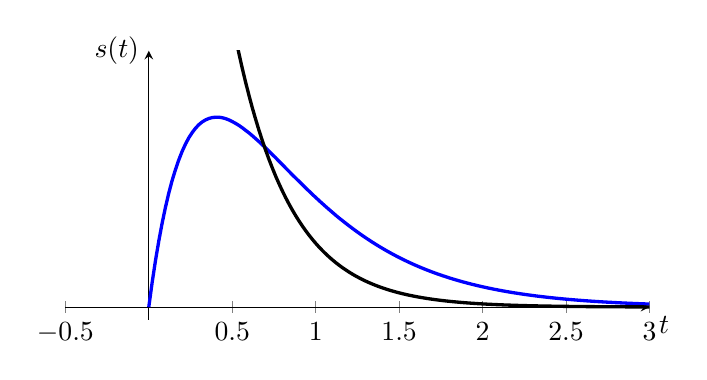
\begin{tikzpicture}
        \begin{axis}[
        scaled y ticks = false,
        height=5cm,
        width=9cm,
        axis x line=center,
        axis y line=center,
        xmin=-0.5,
        xmax=3.0,
        ymin=-0.01,
        ymax=0.2,
        xlabel={$t$},
        ylabel={$s(t)$},
        xlabel style={below right},
        ylabel style={left},
        yticklabels={0,$s(0)=2$},
        ytick={0,2.0},
        y tick label style={anchor=east}
        ]
        \addplot [very thick,color=blue,domain=0:10, samples=501]
        {exp(-2*x)-exp(-3*x)};
        \addplot [very thick,color=black,domain=0:10, samples=501]
        {exp(-3*x)};
        \end{axis}
    \end{tikzpicture}
\end{center}

\newpage
%%%%%%%%%%%%%%%%%%%%%%%%%%%%%%%%%%%%%%%%%%%%%%%%%%%%%%%%%%%%%%%%%%%%%%%%%%%%%%%%
\question{}
%%%%%%%%%%%%%%%%%%%%%%%%%%%%%%%%%%%%%%%%%%%%%%%%%%%%%%%%%%%%%%%%%%%%%%%%%%%%%%%%
\textbf{(3) $\devi{s(t)}{2} + 2\devi{s(t)}{} + s(t)=e(t)$ 
avec $\devi{s(0)}{}=s(0)=0$ et $e(t) = e^{-2t}$}
La transformée de Laplace de l'équation différentielle donne :
\begin{align*}
    p^2S(p)+2pS(p)+S(p)&=E(p) \\
    S(p)&=\dfrac{1}{p^2+2p+1}E(p)
\end{align*}
La fonction de transfert est donné par la fraction rationnelle :
$$
H(p)=\dfrac{1}{p^2+2p+1}
$$
le pôle de $H(p)$ est $p_1=-1$ qui est une racine double
$$
S(p) = \dfrac{1}{(p+1)^2}E(p)
$$
pour $e(t)=e^{-2t}$, $E(p)=\dfrac{1}{p+2}$
$$
S(p)=\dfrac{1}{(p+1)^2(p+2)}
$$
décomposons $S(p)$ en élément simple:
$$
S(p)=\dfrac{A}{p+1}+\dfrac{B}{(p+1)^2}+\dfrac{C}{(p+2)}
$$
$$
A(p^2+3p+2)+B(p+2)+C(p+1)^2=1
$$
$$
\begin{cases}
     A+C&=0 \\
    3A+B+2C&=0 \\
    2A+2B+C&=1
\end{cases}\Longrightarrow
\begin{cases}
    A=-1\\
    B=1\\
    C=1
\end{cases}
$$
$$
S(p)=-\dfrac{1}{p+1}+\dfrac{1}{(p+1)^2}+\dfrac{1}{(p+2)}
$$
la transformée inverse donne :
$$
s(t) = \laplacei{S(p)}= -e^{-t}+te^{-t}+e^{-2t} = (t-1)e^{-t}+e^{-2t}
$$
\begin{center}
\tikzsetnextfilename{ex_3_3_corrige-chap0-ext}
    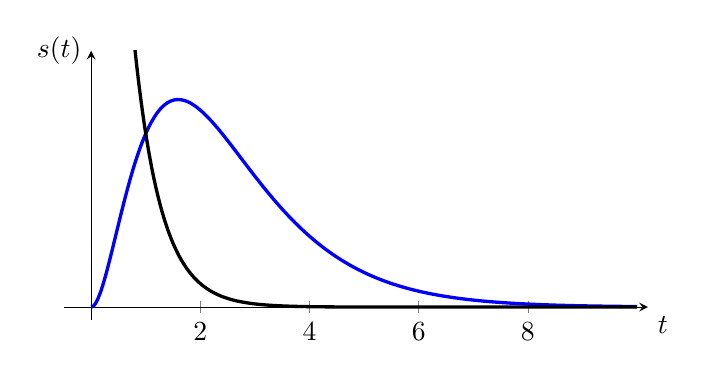
\begin{tikzpicture}
        \begin{axis}[
        scaled y ticks = false,
        height=5cm,
        width=9cm,
        axis x line=middle,
        axis y line=middle,
        xmin=-0.5,
        xmax=10.2,
        ymin=-0.01,
        ymax=0.2,
        xlabel={$t$},
        ylabel={$s(t)$},
        xlabel style={below right},
        ylabel style={left},
        yticklabels={0,$s(0)=2$},
        ytick={0,2},
        xtick={0,2,4,6,8},
        xticklabels={0,2,4,6,8},
        y tick label style={anchor=east}
        ]
        \addplot[very thick,color=blue,domain=0:10 , samples=501]
        {(x-1)*exp(-x)+exp(-2*x)};
        \addplot[very thick,color=black,domain=0:10, samples=501]
        {exp(-2*x)};
        \end{axis}
    \end{tikzpicture}
\end{center}

\newpage
%%%%%%%%%%%%%%%%%%%%%%%%%%%%%%%%%%%%%%%%%%%%%%%%%%%%%%%%%%%%%%%%%%%%%%%%%%%%%%%%
\question{}
%%%%%%%%%%%%%%%%%%%%%%%%%%%%%%%%%%%%%%%%%%%%%%%%%%%%%%%%%%%%%%%%%%%%%%%%%%%%%%%%
\textbf{(4) $\devi{s(t)}{2} + \devi{s(t)}{} + s(t) = e(t)$ 
avec $\devi{s(0)}{}=s(0)=0$ et $e(t) = 1$}}
La transformée de Laplace de l'équation différentielle donne :
\begin{align*}
    p^2S(p)+pS(p)+S(p)&=E(p) \\
    S(p)&=\dfrac{1}{p^2+p+1}E(p)
\end{align*}
La fonction de transfert est donné par la fraction rationnelle :
$$
H(p)=\dfrac{1}{p^2+p+1}
$$
les pôles de $H(p)$ sont deux complexes conjugués: 
$p_{1,2}=-\dfrac{1}{2}\pm j\dfrac{\sqrt{3}}{2}$
$$
S(p) = \dfrac{1}{\left(\left(p+\dfrac{1}{2}\right)^2+
       \dfrac{3}{4}\right)}E(p)
$$
pour $e(t)=1$, $E(p)=\dfrac{1}{p}$
$$
S(p) =\dfrac{1}{p\left(p^2+p+1\right)}
$$
décomposons $S(p)$ en élément simple:
$$
S(p)=\dfrac{A}{p}+\dfrac{Bp+C}{\left(p^2+p+1\right)}
$$
$$
A=\lim\limits_{p \rightarrow 0} pS(p) = 1
$$
\begin{align*}
    p^2+p+1 + Bp^2+Cp &= 1 \\
    \begin{cases}
        B&=-1\\
        C&=-1
    \end{cases}
\end{align*}
\begin{align*}
    S(p)&=\dfrac{1}{p}-\dfrac{p-1}{\left(p^2+p+1\right)} \\
    S(p)&=\dfrac{1}{p}-\dfrac{p}{\left(\left(p+\dfrac{1}{2}\right)^2+
          \dfrac{3}{4}\right)}-
          \dfrac{1}{\left(\left(p+\dfrac{1}{2}\right)^2+\dfrac{3}{4}\right)}\\
    S(p)&=\dfrac{1}{p}-\dfrac{p+\dfrac{1}{2}}
                       {\left(\left(p+\dfrac{1}{2}\right)^2+
                                      \dfrac{3}{4}\right)}-
                       \dfrac{\dfrac{1}{2}}{\left(\left(p+\dfrac{1}{2}\right)^2+
                              \dfrac{3}{4}\right)}\\
    S(p)&=\dfrac{1}{p}-\dfrac{p+\dfrac{1}{2}}
                             {\left(\left(p+\dfrac{1}{2}\right)^2+
                                            \dfrac{3}{4}\right)}-
                       \dfrac{1}{\sqrt{3}}\dfrac{\dfrac{\sqrt{3}}{2}}
                       {\left(\left(p+\dfrac{1}{2}\right)^2+
                                      \dfrac{3}{4}\right)}
\end{align*}
la transformée inverse donne :
$$
s(t) = \laplacei{S(p)}=
1-e^{-\frac{t}{2}}\cos{\left(\dfrac{\sqrt{3}}{2}t\right)}-
\dfrac{1}{\sqrt{3}}e^{-\frac{t}{2}}\sin{\left(\dfrac{\sqrt{3}}{2}t\right)}
$$

\begin{center}
\tikzsetnextfilename{ex_3_4_corrige-chap0-ext}
    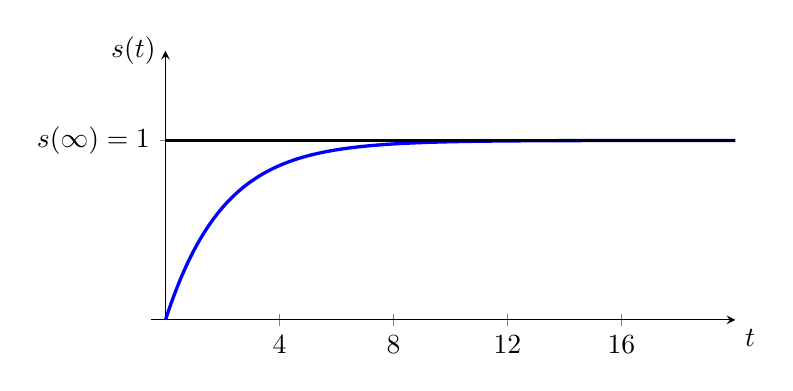
\begin{tikzpicture}
        \begin{axis}[
        scaled y ticks = false,
        height=5cm,
        width=9cm,
        axis x line=center,
        axis y line=center,
        xmin=-0.5,
        xmax=20.0,
        ymin=0.0,
        ymax=1.5,
        xlabel={$t$},
        ylabel={$s(t)$},
        xlabel style={below right},
        ylabel style={left},
        yticklabels={0,$s(\infty)=1$},
        xticklabels={0,4,8,12,16},
        ytick={0,1.0},
        xtick={0,4,8,12,16},
        y tick label style={anchor=east}
        ]
        \addplot [very thick,color=blue,domain=0:20, samples=201]
        {1-exp(-x/2)*cos(sqrt(3)/2*x)-(1/sqrt(3))*exp(-x/2)*sin(sqrt(3)/2*x)};
        \addplot [very thick,color=black,domain=0:20, samples=11]{1};
        \end{axis}
    \end{tikzpicture}
\end{center}

\newpage 
%%%%%%%%%%%%%%%%%%%%%%%%%%%%%%%%%%%%%%%%%%%%%%%%%%%%%%%%%%%%%%%%%%%%%%%%%%%%%%%%
%%%%%%%%%%%%%%%%%%%%%%%%%%%%%%%%%%%%%%%%%%%%%%%%%%%%%%%%%%%%%%%%%%%%%%%%%%%%%%%%
\exercice{Transformée de Laplace d'une fonction périodique}
%%%%%%%%%%%%%%%%%%%%%%%%%%%%%%%%%%%%%%%%%%%%%%%%%%%%%%%%%%%%%%%%%%%%%%%%%%%%%%%%
%%%%%%%%%%%%%%%%%%%%%%%%%%%%%%%%%%%%%%%%%%%%%%%%%%%%%%%%%%%%%%%%%%%%%%%%%%%%%%%%

%%%%%%%%%%%%%%%%%%%%%%%%%%%%%%%%%%%%%%%%%%%%%%%%%%%%%%%%%%%%%%%%%%%%%%%%%%%%%%%%
\question{}
%%%%%%%%%%%%%%%%%%%%%%%%%%%%%%%%%%%%%%%%%%%%%%%%%%%%%%%%%%%%%%%%%%%%%%%%%%%%%%%%
%Déterminer $f_0(t)$ en fonction de $g_0(t)$. 
%Donner la transformée de Laplace de $f_0(t)$.
\tikzsetnextfilename{ex_4_1_corrige-chap0-ext}
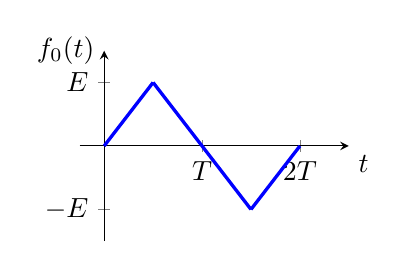
\begin{tikzpicture}
        \begin{axis}[
        height=4cm,
        width=5cm,  
        axis x line=center,
        axis y line=center,
        xmin=-2,
        xmax=20,
        ymin=-1.5,
        ymax=1.5,
        xlabel={$t$},
        ylabel={$f_0(t)$},
        xlabel style={below right},
        ylabel style={left},
        yticklabels={$-E$,$E$},
        ytick={-1,1},
        y tick label style={anchor=east},
        xticklabels={$T$,$2T$},
        xtick={8,16},
        x tick label style={below}
        ]
        \addplot[very thick,color=blue,domain=0:4, samples=101]{0.25*x};
        \addplot[very thick,color=blue,domain=4:12, samples=101]{-0.25*x+2};
        \addplot[very thick,color=blue,domain=12:16, samples=101]{0.25*x-4};
        \end{axis}
\end{tikzpicture}
\tikzsetnextfilename{ex_4_2_corrige-chap0-ext}
\begin{tikzpicture}
        \begin{axis}[
        height=4cm,
        width=5cm,  
        axis x line=center,
        axis y line=center,
        xmin=-2,
        xmax=20,
        ymin=-1.5,
        ymax=1.5,
        xlabel={$t$},
        ylabel={$f_0(t)$},
        xlabel style={below right},
        ylabel style={left},
        yticklabels={$-E$,$E$},
        ytick={-1,1},
        y tick label style={anchor=east},
        xticklabels={$T$,$2T$},
        xtick={8,16},
        x tick label style={below}
        ]
        \addplot [very thick,color=col4,domain=-2:0, samples=101]{0.01};
        \addplot [very thick,color=col4,domain=0:4, samples=101]{0.25*x};
        \addplot [very thick,color=col4,domain=4:8, samples=101]{-0.25*x+2};
        \addplot [very thick,color=col4,domain=8:20, samples=101]{0.01};
        \addplot [very thick,color=col3,domain=-2:8, samples=101]{-0.01};
        \addplot [very thick,color=col3,domain=8:12, samples=101]{-0.25*x+2};
        \addplot [very thick,color=col3,domain=12:16, samples=101]{0.25*x-4};
        \addplot [very thick,color=col3,domain=16:20, samples=101]{-0.01};
        \end{axis}
\end{tikzpicture}
$$
\color{blue}f_0(t)=\color{col4}g_0(t)\color{col3}-g_0(t-T)
$$
où $g_0(t)$ est la fonction \og dent de scie\fg construite précédemment.
$$
F_0(p)=\laplace{f_0(t)}=G_0(p)(1-e^{-Tp})
=\dfrac{2E}{T}\dfrac{(1-e^{-Tp/2})^2}{p^2}(1-e^{-Tp})
$$
\begin{align*}
    F(p)&=\dfrac{F_0(p)}{1-e^{-2Tp}} \\
    F(p)&=\dfrac{2E}{Tp^2}\dfrac{(1-e^{-Tp/2})^2(1-e^{-Tp})}{1-e^{-2Tp}}\\
    F(p)&=\dfrac{2E}{Tp^2}\dfrac{(1-e^{-Tp/2})^2(1-e^{-Tp})}{1-e^{-2Tp}}
                          \dfrac{(1+e^{-Tp})}{(1+e^{-Tp})}\\
    F(p)&=\dfrac{2E}{Tp^2}\dfrac{(1-e^{-Tp/2})^2}{(1+e^{-Tp})}\\
    F(p)&=\dfrac{2E}{Tp^2}\dfrac{(1-2e^{-Tp/2}+e^{-Tp})}{(1+e^{-Tp})}\\
    F(p)&=\dfrac{2E}{Tp^2}\left(1-\dfrac{2e^{-Tp/2}}{(1+e^{-Tp})}\right)
         =\dfrac{2E}{Tp^2}\left(1-\dfrac{e^{-Tp/2}}{e^{-Tp/2}}
                                  \dfrac{2}{(e^{Tp/2}+e^{-Tp/2})}\right)\\
\Aboxed{F(p)&=\dfrac{2E}{Tp^2}\left(1-\dfrac{1}{\cosh{\frac{Tp}{2}}}\right)}
\end{align*}
%%%%%%%%%%%%%%%%%%%%%%%%%%%%%%%%%%%%%%%%%%%%%%%%%%%%%%%%%%%%%%%%%%%%%%%%%%%%%%%%
\exercice{Cartes des pôles et zéros}
%%%%%%%%%%%%%%%%%%%%%%%%%%%%%%%%%%%%%%%%%%%%%%%%%%%%%%%%%%%%%%%%%%%%%%%%%%%%%%%%


%%%%%%%%%%%%%%%%%%%%%%%%%%%%%%%%%%%%%%%%%%%%%%%%%%%%%%%%%%%%%%%%%%%%%%%%%%%%%%%%
%%%%%%%%%%%%%%%%%%%%%%%%%%%%%%%%%%%%%%%%%%%%%%%%%%%%%%%%%%%%%%%%%%%%%%%%%%%%%%%%
%%%%%%%%%%%%%%%%%%%%%%%%%%%%%%%%%%%%%%%%%%%%%%%%%%%%%%%%%%%%%%%%%%%%%%%%%%%%%%%%
%%%%%%%%%%%%%%%%%%%%%%%%%%%%%%%%%%%%%%%%%%%%%%%%%%%%%%%%%%%%%%%%%%%%%%%%%%%%%%%%
%exercice_chap0_corrige.tex
